\documentclass{article}
\usepackage{tikz}
\usepackage{amsmath}
\usepackage{amsfonts}
\usepackage{amssymb}

\begin{document}

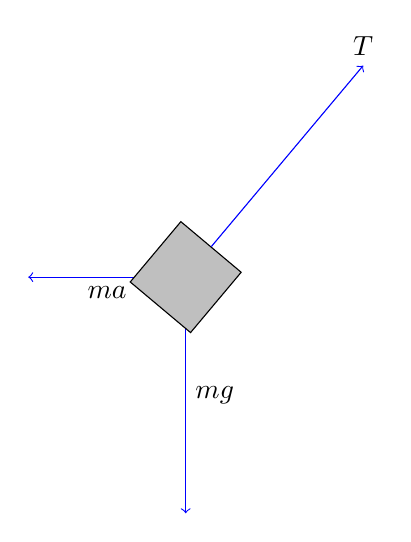
\begin{tikzpicture}[
    force/.style={draw=blue,fill=blue},
    m/.style={rectangle,draw=black,fill=lightgray,minimum size=1cm,thin},
    ]
    \draw[force,->] (0,0) -- (0,-3) node[midway, right] {$mg$};
    \draw[force,->] (0,0) -- (-2,0) node[midway, below] {$ma$};
    \begin{scope}[rotate=50]
    \node[m,transform shape] (M) {};
    \draw[force,->] (M.east) -- ++(3,0) node[above] {$T$};
    \end{scope}
\end{tikzpicture}

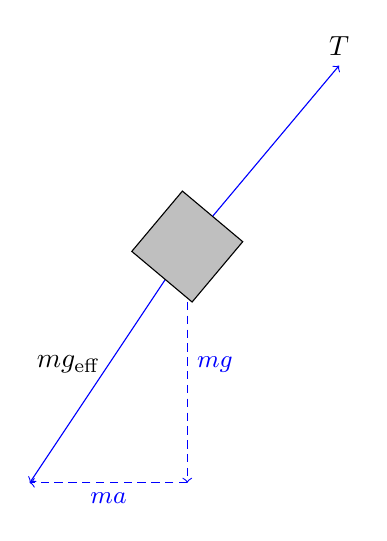
\begin{tikzpicture}[
    force/.style={draw=blue, fill=blue},
    component/.style={densely dashed, blue,font=\small},
    m/.style={rectangle,draw=black,fill=lightgray,minimum size=1cm,thin},
    ]
    \draw[component,->] (0,0) -- (0,-3) node[midway, right] {$mg$};
    \draw[component,->] (0,-3) -- (-2,-3) node[midway, below] {$ma$};
    \draw[force,->] (0,0) -- (-2,-3) node[midway, left] {$mg_\text{eff}$}; 
    \begin{scope}[rotate=50]
    \node[m,transform shape] (M) {};
    \draw[force,->] (M.east) -- (3,0) node[above] {$T$};
    \end{scope}
\end{tikzpicture}

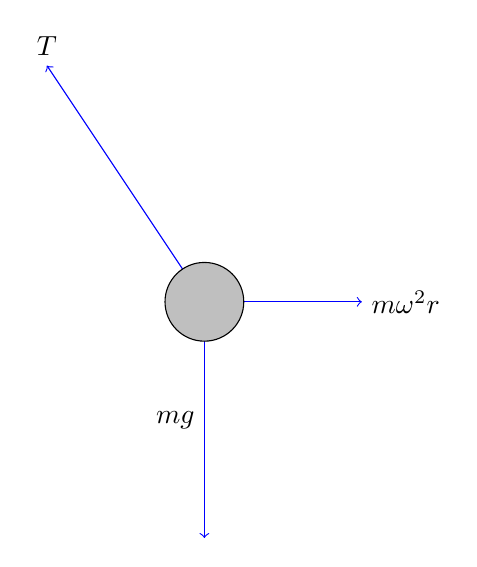
\begin{tikzpicture}[
    force/.style={draw=blue, fill=blue},
    component/.style={densely dashed, blue,font=\small},
    m/.style={circle,draw=black,fill=lightgray,minimum size=1cm,thin},
    ]
    \draw[force,->] (0,0) -- (0,-3) node[midway, left] {$mg$};
    \draw[force,->] (0,0) -- (2,0) node[right] {$m\omega^2 r$};
    \draw[force,->] (0,0) -- (-2,3) node[above] {$T$};
    \node[m,transform shape] (M) {};
\end{tikzpicture}

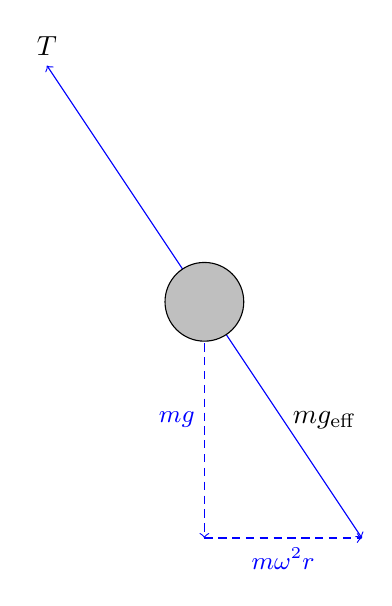
\begin{tikzpicture}[
    force/.style={draw=blue, fill=blue},
    component/.style={densely dashed, blue,font=\small},
    m/.style={circle,draw=black,fill=lightgray,minimum size=1cm,thin},
    ]
    \draw[component,->] (0,0) -- (0,-3) node[midway, left] {$mg$};
    \draw[component,->] (0,-3) -- (2,-3) node[midway, below] {$m\omega^2 r$};
    \draw[force,->] (0,0) -- (2,-3) node[midway, right] {$mg_\text{eff}$}; 
    \draw[force,->] (0,0) -- (-2,3) node[above] {$T$};
    \node[m,transform shape] (M) {};
\end{tikzpicture}

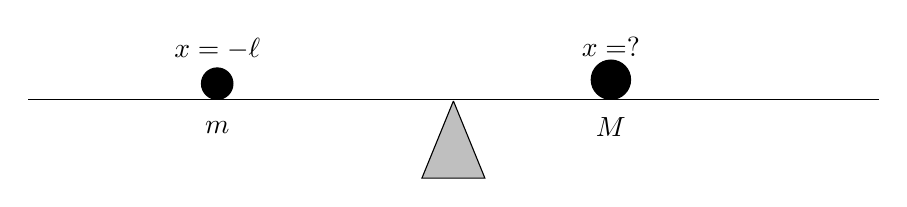
\begin{tikzpicture}
    \draw[](-5.4,1) -- (5.4,1);
    \fill[draw=black,fill=lightgray] (0,0.98) -- (-0.4,0) -- (0.4,0) -- (0,0.98);
    \draw[draw=black,fill=black] (-3,1.2) circle (0.2) node[above, yshift=5] {$x=-\ell$} node[below, yshift=-10] {$m$};
    \draw[draw=black,fill=black] (2,1.25) circle (0.25) node[above, yshift=5] {$x=?$} node[below, yshift=-10] {$M$};
\end{tikzpicture}

\end{document}